\chapter{Methodology} % Main chapter title

\section{Complex networks}
The complex system has several properties. It consists of many components such as units or individuals who interact with each other. The properties of the complex system can not be predicted from the behaviour of one individual. In such systems, without any central force, collective behaviour can emerge. In societies, people's interactions lead to civilisation, economy, formation of social groups or even traffic on the roads. In the animal, populations are present at different levels of the organisation, as in ants and bees colonies or the school of the fishies showing flocking patterns. \cite{boccaletti2006complex}
%latorobook 

The research in complex systems focuses on the structure of the interactions between units. Knowing how branches of the system are connected, we can determine the emergence of the collective behaviour of the system. We can construct networks with neurons and synapses, representing their connections. The structure of the brain network and its properties are fundamental for brain functioning, and neurons in the same brain area are closely connected. Similarly, we can represent the communication between people. The structure of these interactions gives us insights, for example, how information propagates through the system. The presence of people with many connections can lead to faster information flow. 

Despite the differences between complex systems, they can be studied using complex networks; with sets of nodes and edges. Elements in the system are nodes, while interactions between them are given as edges. This approximation allows us to treat equally social (graph of actors), biological (network of proteins) or even technological systems (internet, traffic). In recent years, complex network theory has application in different fields, and the availability of big data incurs its development. \\
%Analyzing and Modeling Real-World Phenomena with Complex Networks: A Survey of Applications
%Characterization of Complex Networks: A Survey of measurements

The complex network theory originates from the graph theory in mathematics. These days, the graph and network are used as equivalent terms. The first mathematical problem solved using graph theory was $Konigsberg$ problem of seven bridges. The city $Konigsberg$ had seven bridges connecting the city's parts across the river and the island in the middle. The question was, is it possible to find a walk that crosses all seven bridges only once. Representing the problem as a graph, Euler managed to simplify the problem; the parts of the land are represented as nodes while bridges between them are links. Crossing each bridge only once is possible if each part of the land has an even number of connections. Thus, it was not possible in this case, as each piece of land had an odd number of bridge connections, see Fig. \ref{fig:Krgraph}.

\begin{figure}[h!]
	\centering
	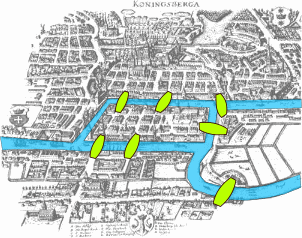
\includegraphics[width=0.3\linewidth]{Figures/Konigsberg_bridges.png} \hspace{2cm}
	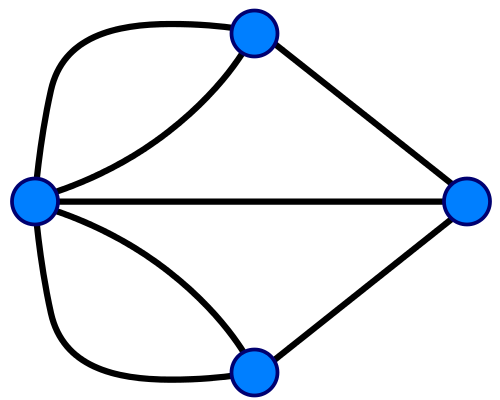
\includegraphics[width=0.3\linewidth]{Figures/Konigsberg_graph.png}
	\caption{The Kronigsber problem of seven bridges.}
	\label{fig:Krgraph}
\end{figure}

\section{Types of networks}

%The seven bridges problem in Fig. \ref{fig:Krgraph} is represented with the \textbf{simple network} structure. 
The graph or network $G$ is defined as $G=(V, E)$, where $V$ is a set of nodes (vertices), and $E$ is a set of edges. The edge is pair of nodes $e_{ij} = (i, j), $ and $i,j\in E$. The graph structure has undirected edges meaning that edges are symmetric: $(i, j)$ implies $(j, i)$. Edges are also unweighted, meaning that all edges are equally important. The specific properties of the nodes are also neglected in this representation. The \textbf{adjacency matrix} ${A} = N \times N$ has value $1$ if there is connection between two nodes, otherwise it is $0$ \cite{boccaletti2006}\\

For example, if we consider unweighted, undirected network, with only 3 nodes and two connections, adjacency matrix is:


\begin{equation}
A = \begin{bmatrix}
0 & 1 & 1\\
1 & 0 & 0 \\
1 & 0 & 0 \\
\end{bmatrix}
\end{equation}

The self loops usually are not considered, meaning that $A_{ii}=0$. 
%The complex system can be represented by complex network $G=(V, E)$, where the elements of system (atoms, proteins, people) map to set of $N$ nodes $V=\{1, 2, ...,N\}$. The interactions between elements map to $L$ links between nodes, $E = \{ e_1, e_2... e_L\}$. The \textbf{adjacency matrix} ${A} = N \times N$ has value $1$ if there is connection between two nodes, otherwise it is $0$ \cite{boccaletti2006}.

Other equivalent way of representing graph is as edge list. Instead of having adjacency matrix, graph is described with the list of links that are in graph. The graph is then pair of $N, g$, where N is set of nodes, and $g$ is collection of links, listed as subset of $N$ of size 2. So the network is written as $g = \{ \{1,2\}, \{2,3\}\}$.

Sometimes it is essential to include specific properties of the system in the network representation, which can help create more realistic models. The additional properties can be added on the edge, node or network level. \\

\begin{figure}[h!]
	\centering
	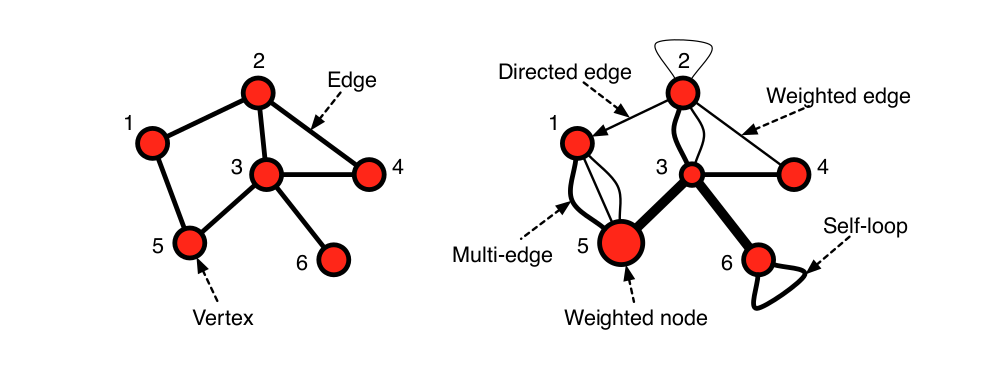
\includegraphics[width=1\linewidth]{figures/methodology/graph1.png} 
	\caption{Graph types}
	\label{fig:gt1}
\end{figure}

In a \textbf{directed network}, edges have broken symmetry. The interaction from node $i$ to node $j$ does not need to have the same property as the interaction from node $j$ to node $i$. A typical example is WWW, where webpages are nodes, and hyperlinks are directed edges. In biological networks, gene regulation and neural activation can be given as directed networks. \\ %clasuet networks

\begin{figure}[h!]
	\centering
	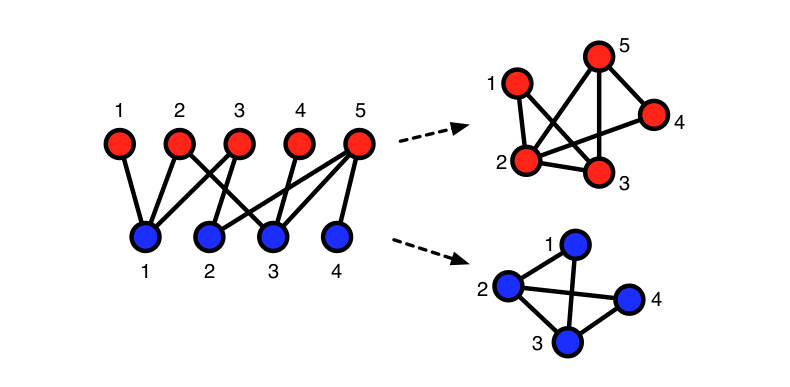
\includegraphics[width=0.8\linewidth]{figures/methodology/graph2.png} 
	\caption{Graph types}
	\label{fig:gt2}
\end{figure}

The frequency of interaction between nodes is emphasised if edges are associated with different scalar values; networks are \textbf{weighted}. The edges may be signed, representing activation in the biological system or trust and distrust in the social system. In general, edges can be associated with any categorical variable. If attribute describes the time when an interaction between nodes happened; network is called \textbf{temporal}. Finally, \textbf{multigraph} allows the presence of multiply edges between two nodes. For the network between cities, edges may be different driving paths between them. In neuron cells, multiply synapses are represented as distinct edges. \\

A \textbf{bipartite network} has two partitions, $U$ and $V$. The nodes in the same partition are not connected while links exist only between nodes of a different kind. In general, we can define k-bipartite graph. The set of nodes $V$ has $k$ distinct classes of nodes. When $k=2$ the network is bipartite.  Bipartite networks represent the membership of people or items in groups. For example, we can define the network of actors as a bipartite graph. In one partition are actors and in other movies. There are no edges between actors or movies, but the actor is connected to the film if it plays in that movie. Another example is a recommender network, such as a network of people and items they like. 

The equivalent representation of bipartite network is incidence matrix $B$. If $n$ is number of people and $g$ number of groups, this matrix is $g x n$, having elements $B_{ij}$ 1 if persoon i belongs to group j. 

Even bipartite networks give realistic representation of the system, there is often need to analyze the single type of nodes.  From a bipartite network, we can generate two projections. The first one connects nodes partition $V$ if they point to node $u$. Similarly, we can project the network on U partition, connecting $u$ nodes. The one mode projection between actors and movies onto actors is undirected network of actor collaborations. Actors are connected if they appear in the same movie. We can also create one-mode projection onto movies, where two movies are connected if they share the same actor.  

The projections are useful in some manner, but they also lose some important information, for example how many groups nodes share in common. This information can be propagated adding the weight to the edges, equal to the number of common groups.

The product $B_{ki}$ and $B_{kj}$ is 1 if $i$ and $j$ belong to the same group $k$. Thus the total number of groups to which nodes $i$ and $j$ belong is $P_{ij} = \sum_{k=1}^g B_{ki}B_{kj} = \sum_{k=1}^g B_{ik}^TB_{kj}$. The matrix $P$ is matrix of one-mode projection. The diagonal elements are non-zero, and represent the number of groups node $i$ belongs to.  To derive the weighted adjacency matrix, the diagonal elements are set to 0. The adjacency matrix of unweighted projection, each non-zero element needs to be replaced with $1$. 

The important consequence of the one-mode projection is the construction of the cliques; subgraph in which every pair of nodes is connected. Every node that is being projected is represented as a clique of size, because all pairs of its neighbours are exactly distance two away from each other. All actors in the movie will be joined in a clique in the one-mode actor projection. %ovo preformulisati

Another consequence of the one-mode projection is that one mode projection may originate from different bipartite networks. Meaning that projection is not one-to-one; no bijection. It is surjective operation, meaning hat any projected network $P$ has at least one bipartite network such that the projection of B results in P. \\ %ovo preformulisati

\begin{figure}[h!]
	\centering
	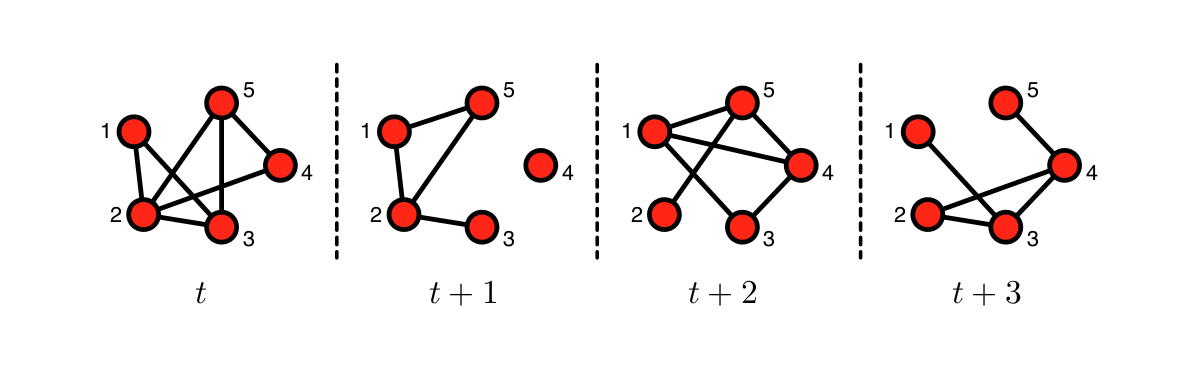
\includegraphics[width=1\linewidth]{figures/methodology/graph4.png} 
	\caption{Graph types}
	\label{fig:gt3}
\end{figure}

In \textbf{temporal networks} nodes and edges evolve. Many real networks are not static, networks grow over time, and edges and nodes may emerge or disappear. Also, some edges may be active at regular intervals, reflecting the circadian rhythms of the nodes. In citation networks, new nodes (paper) join the network, creating links with cited papers. 

Let consider the temporal network with $N$ nodes, over time interval $t_{max}$. The event representation consists in viewing the temporal networks as a collection of time-stamped edges. In this representation, each edge $(i, j)$ is defined as$(i, j, t, \Delta t)$, where $t$ is the time of the event and $\Delta t$ its duration. In a temporal network, the same link can appear multiple times, and the duration of the event may vary. An example of an event temporal network may be phone-calls networks, where a call between two persons $i$ and $j$ started at time $t$ and ended at $t + \Delta t$. 

A temporal network can be represented as sequence of networks $G= G(1), ... G(t_{max})$, where $t_{max}$ is number of networks. While in the event-based representation, time can be both discrete and continuous, in the snapshot representation, time is only discrete. The temporal network is seen as a structure that evolves in time, and at each timestamp, we can analyse the system's macroscopic properties. We need to specify time windows for coarse-grain event-based representation of the temporal information in the data. If we use uniformly time window of length $w$ then the events occurring in $0 \leq t < w$ enter snapshot G(1), those occurring in $w \leq t < 2w$ enter G(2) and so forth. We can not recover the original data points from the snapshot representation, and more information loss is present with a larger time window. If the time window is $w=t_{max}$, there is only one snapshot, temporal data are no more available, and the network is static. \\

\begin{figure}[h!]
	\centering
	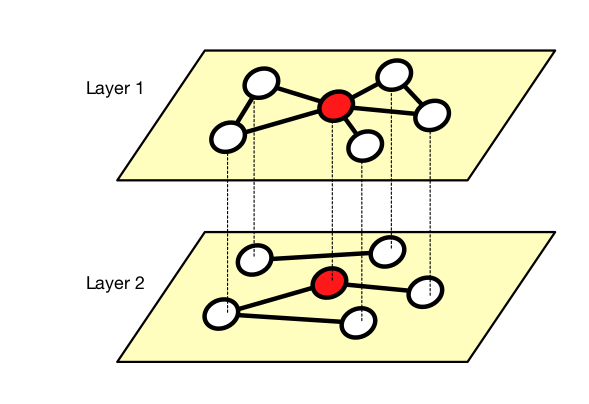
\includegraphics[width=0.5\linewidth]{figures/methodology/graph5.png} 
	\caption{Graph types}
	\label{fig:gt5}
\end{figure}

A network in which edges are marked by which "layer" they exist in is called a multiplex or multilayer network. These networks are used to represent a system in which there are multiple types of interactions, and we store the connectivity of each kind in a different "layer" of the multiplex network. A temporal network is a special kind of multiplex network, where these layers form a temporal (ordered) sequence. Crucially, there can dynamics on each vertex that govern which layer some kind of interaction occurs on, so multiplex networks are not merely a special kind of graph in which different colors or layer numbers annotate edges. %clauset preformulisati

Spatial networks are a special kind of node-annotated network, in which the annotations represent the node's location in some d-dimensional space. This graph property is most common in transportation networks, e.g., as road and city networks, airport transportation networks, oil and gas distribution networks, shipping networks, etc., but can also appear in social networks. Planar graphs are a special case of spatial networks in which the nodes are embedded on a 2-dimensional surface and edges do not cross. %clauset preformulisati

Hypergraphs are another type of network, in which edges denote the interaction of more than two vertices, e.g, E in V × V × V . Scientific collaboration graphs can be represented as a hypergraph, in which each "edge" is the set of coauthors on a scientific article. However, collaboration networks are more commonly represented as bipartite graphs, in which scientists and papers form two sets of vertices, and scientist-nodes are connected to all the paper-nodes on which they are authors. %clauset to do

%The canonical network form is an undirected graph, where two nodes are either connected or not. This applies to situations where two nodes are either in a relationship with each other or not, but it cannot be that one is related to the second without the second being related to the …rst. This is generally true of many social and/or economic relationships, such as partnerships, friendships, alliances, acquaintances, etc. This sort of network will be central to most of the chapters that follow. However, there are other situations that we will examine that are better modeled as directed networks, where one node may be connected to a second without the second being connected to the …rst. For instance, a network that keeps track of which authors cite which other authors, or which web pages have links to which others would naturally take the form  of a directed graph.

\section{The structure of complex networks}

\subsection{Paths and cycles}

As network is connected structure, the nodes may be influenced also by distant nodes, and the information might spread through the links of a network. Analyzing the paths of the network is important task.   

A path of the network between two nodes $i$ and $j$ is a sequence of links, $i_1i_2,..,i_k$ such $i_ki_{k+1} \in g$ that $i_1=i$ and $i_k=j$, each node in the sequence is distinct. 
The path is walk, if nodes in the sequence are not distinct, so walk can visit one node more than once. The cycle is walk that starts and ends at the same node, while other nodes are distinct. 

Note that, if we use adjacency matrix representation where $A_{ii}=0$, then $A^2$ tells us how many walks of length 2 exist between any two nodes.

Network is connected if every two nodes in the network are connected by some path. So the network is connected id for every node $i \in N$ and node $j \in N$ exists a path between them. 

A component of the network are distinct maximal connected subgraphs of a network. In the example there are 4 components. Note that in this definition of the component isolated node is also component. In directed network, set of nodes that are reachable from each other is a strongly connected component, while a set of nodes where either i is reachable from j or j is reachable from i is weakly connected component.

There are a few particular network structures that are commonly referred to.
A tree is a connected network that has no cycles.
A forest is a network such that each component is a tree. Thus any network that
has no cycles is a forest, as in the example pictured in Figure 2.1.6.
A particularly prominent forest network is a star. A star is a network such that
there exists some node i such that every link in the network involves node i. In this
case i is referred to as the center of the star.
There are a few facts about trees that are easy to derive (see Exercise 2.2) and
worth mentioning.
A connected network is a tree if and only if it has n
1 links.
A tree has at least two leaves, where leaves are nodes that have exactly one link.
In a tree, there is a unique path between any two nodes.
The complete network is one where all possible links are present, so one where
where g ij = 1 for all i 6 = j.

A circle (also known as a cycle-graph) is a network that has a single cycle and such
that each node in the network has exactly two neighbors.
In the case of directed networks, there can be many di¤erent stars involving the
same set of nodes and having the same center, depending on which directed links are
present between any two linked nodes. On occasion, it will be useful to distinguish
between these.

Eulerian tours and Hamiltonian cycles

A walk is said to be closed if it starts and ends at the same node. It is clear that in
order to have a closed walk that involves every link of a network exactly once it must
be that each node in the network has an even degree. 39 This follows since each time a
node is “entered” by one link on the walk it must be “exited”by a di¤erent link, and
each time the node is visited, it must be by a link that has not appeared previously on
the walk. Euler’s [?] simple but remarkable theorem is that this condition is necessary
and su¢ cient for there to exist such a closed walk.

A connected network g has a closed walk that involves each link ex-
actly once if and only if the degree of each node is even.


One can ask a related question for nodes rather than links: when is it possible to
…nd a closed walk that involves each node in the network exactly once? Such a closed
walk must be a cycle, and is referred to as a Hamilton Cycle or a Hamiltonian. A
related question is whether there exists a “Hamilton path”that hits each node exactly
once. Clearly a network that has a Hamilton cycle has a Hamilton path, while the
converse is not true (consider a line).
Discovering whether or not a network has a Hamilton cycle is a much more chal-
lenging question than whether it has a Euler tour; and this has been an active area
of research in graph theory for some time. It has direct applications to the “traveling
salesman problem,”where a salesman must visit each city on a trip exactly once, cities
are nodes on a network, and the path must follow the links.
The seminal theorem on Hamilton cycles is due to Dirac [?]. Stronger theorems
have since been developed, as we shall shortly see, but it is worth stating on its own,
as it has an intuitive proof that helps one see the paths to proving some of the later.

\subsection{Community structure}

\subsection{Core-periphery structure} 

\section{The network analysis}

%The complex system can be represented by complex network $G=(V, E)$, where the elements of system (atoms, proteins, people) map to set of $N$ nodes $V=\{1, 2, ...,N\}$. The interactions between elements map to $L$ links between nodes, $E = \{ e_1, e_2... e_L\}$. The \textbf{adjacency matrix} ${A} = N \times N$ has value $1$ if there is connection between two nodes, otherwise it is $0$ \cite{boccaletti2006}. 

\subsection{Degree distribution}

The simplest network measure is \textbf{node degree}, $k$. The degree of node $i$ gives the number of nodes attached to node $i$, $k_i = \sum_j A_{ij}$. 

The density of the network is average degree divided by $N-1$, where $N$ is number of nodes. It is relative fraction of nodes in the network. 

In the case of regular networks, such as grids, each node has an equal degree, meaning that nodes in the network have similar roles. In the general case, the networks have more complicated structure. If degree sequence is skewed, we are able to identify nodes with high degree, hubs. Removing hubs may partition a connected network into several components. Finally, if we are able to test isomorphism between two graphs, the starting point would be to compare their degree sequences are the same. If they are not, then they can not be isomorphic. \\

To calculate the degree distribution we can consider the fraction of $k$ degree nodes $N_k$, $p(k) = N_k/N$. It is the probability , $P(k)$, that randomly chosen node has degree $k$. Similarly, we can order nodes according to their degree and plot the node degree. \\

If the nodes of the graph are statistically independent, the degree distribution completely determines the properties of a network. If degree distribution is present $P(k)$, and the total number of nodes is fixed to $N$. We can construct a graph with random connections. Label N vertices. To node $j$ of the graph ascribe degrees $k_j$, taken from the distribution $P(k)$. Connect at random ends of pairs of distinct quills belonging to distinct vertices. 

\begin{itemize}
	\item The Poisson distribution. The degree distribution in random network, where all nodes have the same connecting probability, follows Poisson distribution $P(k)= \frac{(Np)^ke^{-Np}}{k!}$, where $k$ is the mean degree distribution. 
	
	\item Exponential distribution. $P(k) = e^{-k/ \- k}$. This is degree distribution of the growing random graph. Even for infinite networks all moments of distributions are finite, and have natural scale of the order of average degree.
	
	\item In real networks degree distribution follows a power law. $P(k) = k ^ {-\gamma} $, where $\gamma$ is exponent of the distribution. In this distribution there is no natural scale, so they are called scale-free networks. In infinite networks all higher moments diverge. If the average degree of scale-free networks is finite, than $\gamma$ exponent should be greater than 2. Therefore, real networks have a scale-free structure with the emergence of the hubs \cite{newman2010}. In finite size networks, fat-tailed degree distributions have natural cut-offs. 
\end{itemize}

 \begin{figure}
 	\centering
 	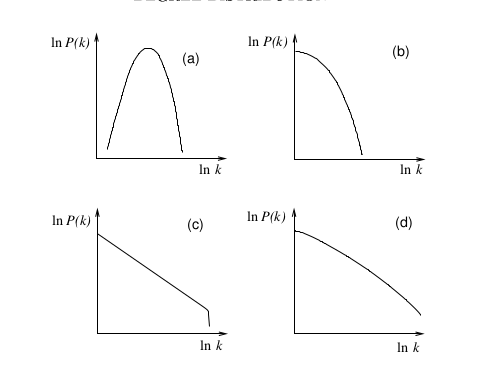
\includegraphics[width=0.5\textwidth]{figures/methodology/distributions.png}
 	\caption{Distributions, ovde hocemo 3 distribucije+ linearna vs. logarithm scala, takodje pokazati kako izgleda frequency order}
 	\label{fig:dist}
 \end{figure}

When plotting the degree distribution, it is common to use scaling of the axis. As explained, we rank the nodes according their degree and plot the node degree of each kth node. In the first example, we used linear scale for both axes. As many nodes have  low degree, it is more useful to use logarithmic scale. On the logarithmic scale the distance between two points is proportional to the logarithm of distance between two points, meaning that distance on logarithm scale is same between points 10 and 100, and 100 and 1000.  Now it is more easily notices that data-points follow straight line, meaning that degree distribution is some kind of exponential function. 

\subsection{Degree correlations}

Correlation is defined through a correlation coefficient r. If x and y are two stochastic variables, for which we have a series of observation pairs $(x_1, y_1), (x_2, y_2), ... (x_n, y_n)$. The correlation coefficient $r(x, y)$ between $x$ and $y$ is defined as:

\begin{equation}
r(x, y) = \frac{\frac{1}{n}\sum_{i=1}^{n}((x_i - \bar{x} ) (y_i - \bar{y}) )}{\sqrt{\frac{1}{n}\sum_{i=1}^{n}(x_i - \bar{x})^2} \sqrt{\frac{1}{n}\sum_{i=1}^{n}(y_i - \bar{y})^2} }
\end{equation}

where $\bar{x} = \frac{1}{n}\sum_{i=1}^{n}x_i$, is the average over variable $x$. \\

Taking the definition of correlation coefficient we can define it for vertex degrees. For simple graph G with vertex set $V(G) = \{v_1, ..v_n\}$, $\boldsymbol{A}[i,j] = 1$ if there is a link between nodes $v_i$ and $v_j$. If G is a simple graph with adjacency matrix $\boldsymbol{A}$ and degree sequence $\boldsymbol{d} = [d_1, ..., d_n]$

\begin{equation}
r_{deg}(G) = \frac{\sum_{i=1}^{n}\sum_{i=1+1}^{n}((d_i - \bar{d}) (d_i - \bar{d}) \boldsymbol{A}[i,j] )}{\sum_{i=1}^{n}(d_i - \bar{d})^2}
\end{equation}

Using adjacency matrix, allow us to calculate the correlations between neighboring nodes. If two nodes are not connected $A[i,j]=0$, the degree correlation between them do not have contribution to the $r$.

The \textbf{degree-degree correlations} in the network are measured by \textbf{assortativity}. If correlations are positive, networks are assortative; there is a tendency that connections exist between similar degree nodes. The negative correlations indicate that large degree nodes have preference to connect nodes with small degree; dissasortative networks. The average first neighbor degree $k_{nn}$ can be calculated as $k_{nn} = \sum_{k^{'}}k^{'}P(k^{'}|{k})$. The $P$ is conditional probability that an edge of degree $k$ points to node with degree $k$. The norm is $\sum_{k^{'}}P(k^{'}|k)=1$, and detailed balance conditions \cite{boccaletti2006},  $kP(k^{'}|k)P(k) = k^{'}P(k|k^{'})P(k^{'})$ \cite{boccaletti2006}. If the node degrees are uncorrelated, $k_{nn}$ does not depend on the degree, otherwise increasing/decreasing function indicates on positive/negative correlations in the network. \\

The Newman defined the assortativity index $r$ in slightly different way:

\begin{equation}
r = \sum_{kl}kl(e_{kl} - q_lq_k) / \sigma_q^2
\end{equation}

where $e_{kl}$ is the probability that randomly selected link connect nodes with degrees $k$ and $l$, $q_k$ is probability that randomly choosen node is connected to node $k$ and equals $q_k = kp_k / \langle k \rangle$, while $\sigma_q$ is variance of the distribution $q_k$. 

\subsection{Distances}

Between two nodes in the network, we can define different paths, but the most important one are the shortest paths. The distance between two nodes $d(i, j)$ is defined as the length of shortest path between two nodes. 
In the case of weighted networks, is defined such that the path has minimal weight, and the length of such path does not have to be minimal. Distances on the network, again can give us insight how to networks are similar, and to give indication of relative importance of the node in the network. 

The eccentricity of the vertex, gives us how far the farthest vertex is positioned in the network. The radius is minimum over all eccentricity values, while the diameter defines the largest distance between nodes in the network. These definitions apply to directed and undirected graphs. 

The diameter gives us useful information, it may not be powerful enough to discriminate among graphs. An important metric is to consider the distribution of path lengths. The average distance between nodes is useful for network description. 

If G is connected graph with vertex set V and $\bar{d}(u)$ is average length of the shortest paths from node u, to any other node v in network G.

\begin{equation}
\bar{d}(u) = \frac{1}{|V|-1} \sum_{v\in V, v \notin u} d(u,v)  
\end{equation}

From there we can define the average path length as mean value over $\bar{d}(u)$.

\begin{equation}
\bar{d}(G) = \frac{1}{|V|}\sum_{u \in V} \bar{d}(u)
\end{equation}



 while the characteristic path length of G is median over all $\bar{d}(u)$.


\subsection{D-measure}

%Between two nodes in the network, we can define different paths, but the most important one are the shortest paths, $d_{ij}$. Diameter defines the largest shortest path found in the network. 

For each node $i$ we can define the distribution of the shortest paths between node $i$ and all others nodes in the network, $P_{i}=\{p_{i}(j)\}$, where $p_{i}(j)$ is percent of nodes at distance $j$ from node $i$. The connectivity patterns can efficiently describe difference between two networks.    
To specify how much $G$ and $G^{'}$ are similar we use D-measure \cite{tiago2}
\begin{equation}
D(G, G^{'}) = \omega \left| \sqrt{\frac{J(P_1,..P_N)}{log(d)}}-\sqrt{\frac{J(P_1^{'},..P_N^{'})}{log(d^{'})}} \right| + (1-\omega) \sqrt{\frac{J(\mu_{G},\mu_{G^{'}})}{log2}}
\label{eq:dmeasure}
\end{equation}

D-measure calculates Jensen-Shannon divergence between $N$ shortest path distributions,

\begin{equation}
J(P_1,.., P_N)) = \sum_{i,j}p_i(j)log(\frac{p_i(j)}{\mu_j})
\end{equation}

where  $\mu_j = (\sum_{i=1}^N p_i(j))/N$ is mean shortest path distribution. \\

The first term in equation \ref{eq:dmeasure} compares local differences between two networks, and Jensen-Shannon divergence between $N$ shortest path distributions $J(P_{1},...,P_{N})$ is normed with network diameter $d(G)$. The second part determines global differences, computing  ${J(\mu_{G},\mu_{G^{'}})}$ between mean shortest path distributions. 
%We consider equally important local and global properties of the networks, and parameter $\omega$ is set to $0.5$. 
The D-measure ranges from $0$ to $1$. The lower D-measure is, networks are more similar and for D-measure $D = 0$, structures are isomorphic.

%OVDE mozda neka slika d-mere da bude intuitivnije kako radi

\subsection{Clustering coefficient}



%A common way toward spreading information is simply having a node update its neighbors. In turn, neighbors can inform their neighbors, and so on. There are many variations to this model, such as having a node select only one or a few of its neighbors, or deciding to stop spreading updates when it notices that a selected neighbor already has the information. Informally, this type of dissemination is often described in the form of gossiping models, also known as epidemic dissemination [Eugster et al., 2004]. The model is very general: instead of information we can also consider spreading of diseases, but also viruses over the Internet. Another example is that of forming of opinions, which often depends on what the majority of your community thinks. We shall return to these issues in more detail when discussing peer- to-peer networks in Chapter 8.

%When considering real-world networks, we often see that they are organized as a collection of interconnected groups. In terms of social networks, this means that we can often clearly distinguish communities of nodes with many links between its members, yet relatively few links between nodes that belong to different communities. Actually indicating which nodes belong to which communities may not be easy at all. Also, nodes generally belong to more than one community. However, we can express the existence of communities by means of a clustering coefficient. As shown by Xu and Liu [2008], it turns out that there is a clear relationship between the speed by which information is disseminated in social networks and the clustering coefficient: the higher the degree of clustering, the slower the dissemination. To a certain extent, this result may seem quite obvious, but from a formal (i.e., mathematical) point of view, it turns out to be not so trivial. What this means is that if we want to design a dissemination protocol, we may need to take special measures in highly clustered networks in order to guarantee a certain performance regarding the dissemination speed. This alone has been enough reason for researchers to define and measure the clustering coefficient of a network. Besides this reason, measuring the clustering coefficient obviously alows us to simply compare different networks, without necessarily wanting to make use of the actual values of the respective coefficients. In this sense, clustering coefficients can help in classifying networks.

The \textbf{clustering coefficient} is a measure describing the neighbourhood's structure. In networks exist tendency to form triangles or clusters. This is common in friendship networks where two friends of one person have a high probability of being friends. The clustering can be measured by computing the number of links between neighbours of one node,
\begin{equation}
c_i=2e_i/(k_i(k_i-1))
\end{equation}

Averaging it over all network nodes, we can calculate the mean clustering coefficient. It ranges from  $\langle c \rangle = 0$ where connections between neighbouring nodes do not exist, network has the structure of three. On the other hand, $\langle c \rangle = 1$ indicates a fully connected network. \\

Newman proposed the alternative definition for the clustering coefficient based on the number of triples and triangles in a graph. A triangle at node $v$ is complete subgraph with 3 nodes, including $v$. A triple on the node v is a subgraph of exactly three nodes and two edges, where v is incident with two edges. The network transitivity is defined as the ratio of number of triangles in the network over the number of triples. The network transitivity is seen as global clustering, as it considers the whole network.  


%n the network literature we ocassionally encounter the global cluster- ing coefficient, which measures the total number of closed triangles in a network. Indeed, L i in (2.15) is the number of triangles that node i partic-ipates in, as each link between two neighbors of node i closes a triangle (Figure 2.17). Hence the degree of a network’s global clustering can be also captured by the global clustering coefficient, defined as 

%where a connected triplet is an ordered set of three nodes ABC such that A connects to B and B connects to C. For example, an A, B, C triangle is made of three triplets, ABC, BCA and CAB. In contrast a chain of connected nodes A, B, C, in which B connects to A and C, but A does not link to C, forms a single open triplet ABC. The factor three in the numerator of (2.17) is due to the fact that each triangle is counted three times in the triplet count. The roots of the global clustering coefficient go back to the social network literature of the 1940s [17, 18], where C Δ is often called the ratio of transitive triplets.

\subsection{Real-world networks}
Real-world networks share similar properties. The mean distance between nodes is smaller than the number of nodes in the network $l << N$, called small-world phenomena. This cause the fast spread of information or even diseases in the complex systems. In small-world networks number of vertices grow exponentially with distance; thus $l$ increase as $log(n)$ or slower. Logarithmic scaling can be proved from various network models; also, it is observed in real-world complex systems. The clustering coefficient in real-world networks is usually high. Real-world networks have one important feature; power-law degree distribution; such networks are called scale-free networks.

\newpage
\section{Network models}

\subsection{Random network model}

The random graph model was introduced by mathematicians Paul Erdős and Alfred R\' {e}nyi in 1959. In this model, connections between nodes are chosen randomly, and every link has the same probability of existing. The graph is characterized only by a number of the nodes $N$ and the linking probability $p$, so Erdős-R\' {e}nyi graph is written as $G(n, p)$. \\

The creation of ER random network consists of the following steps:
\begin{itemize}
	\item we start with $N$ isolated nodes
	\item between each $N(N-1)/2$ pair of nodes we create link with probability $p$; sampling random number $r \in (0,1)$, we create link if $r \leq p$    
\end{itemize}


\begin{figure}[h!]
	\centering
	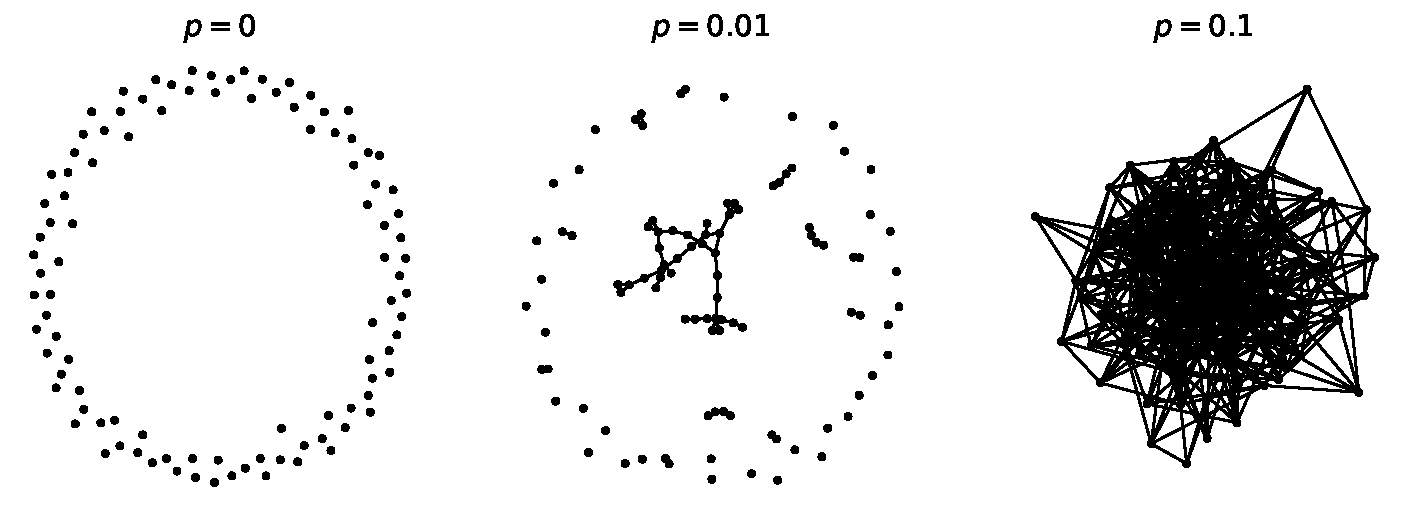
\includegraphics[width=0.9\linewidth]{figures/methodology/ERgraph}
	\caption{ER graph with $N=100$ nodes and different linking probabilities $p$.}
	\label{fig:erp}
\end{figure}

We should note that this process is stochastic. The networks $G(N, p)$ with the same parameters do not need to have the same structure; i.e. they differ in the number of links. Therefore, the single random graph is only one graph from all the possible realizations in the statistical ensemble. 

Two simple quantities that could be estimated are the average number of links and the average degree. For complete graph with $N$ nodes, number of edges is $N(N-1)/2$. As the probability of drawing every edge is $p$, the \textbf{average number of links} is simply given as 

\begin{equation}
\langle L \rangle = \frac{N(N-1)}{2}p
\end{equation}

From there, we conclude that the network's density is equal to probability $p$.
The \textbf{average degree} is approximated as: $\langle k \rangle = 2 \langle L \rangle / N $, leading to:

\begin{equation}
\langle k \rangle = (N-1)p 
\end{equation}

The \textbf{degree distribution} of ER random graph follows the binomial distribution. 

\begin{equation}
P(k) = \binom{N-1}{k}p^k(1-p)^{N-1-k}
\end{equation}

The probability that the node has degree $k$ is given with the second term $p^k$, while the probability that other N-1-k links are not created is given with the third part of the equation. Finally, there are  $\binom{N-1}{k}$ combinations for one node, to have $k$ links from $N-1$ possible links. 

The binomial distribution describes very well small networks. For larger networks, we find that they are sparse and that the average degree is much smaller than a number of nodes $\langle k \rangle << N$. In this limit, binomial distribution becomes the Poisson, which now depends only on one parameter $\langle k \rangle$

\begin{equation}
p(k) = \frac{1}{k!}e^{-\langle k \rangle}\langle k \rangle^{k}
\end{equation}

\begin{figure}[h!]
	\centering
	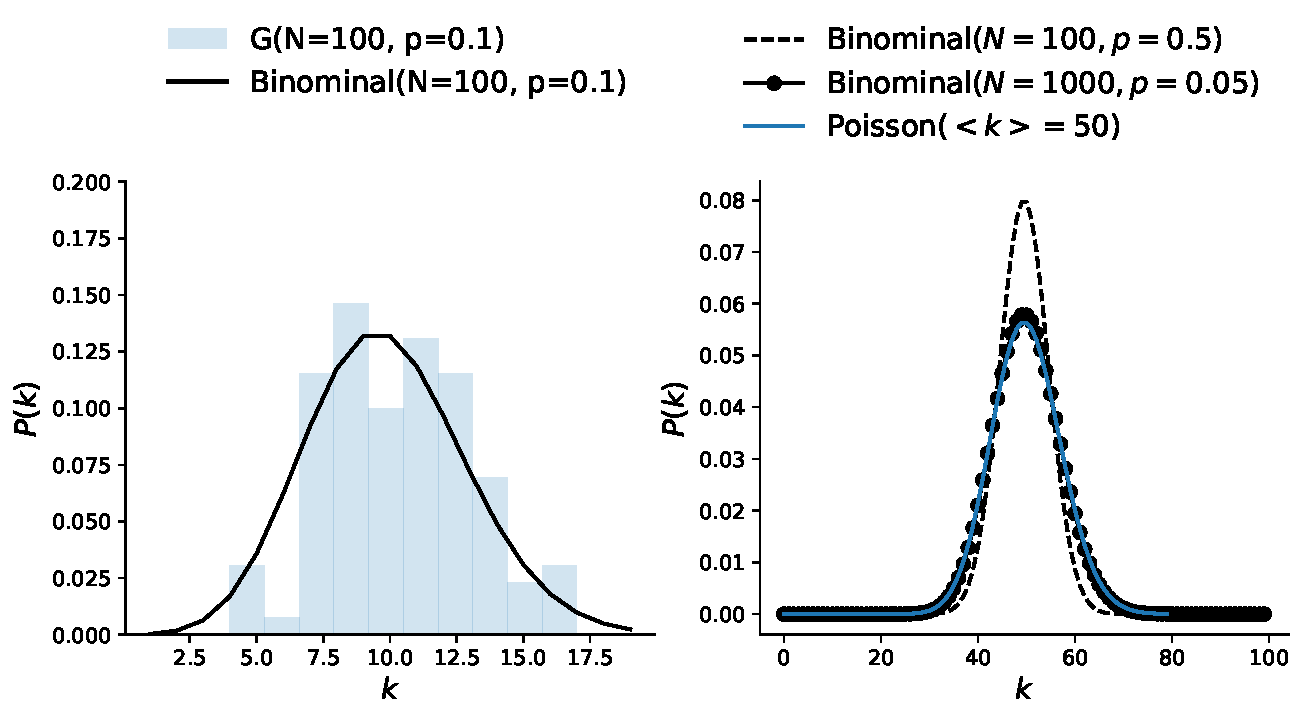
\includegraphics[width=0.9\linewidth]{figures/methodology/ER_dist}
	\caption{Degree distribution of ER graph. Degree distribution of small networks follow binominal. Larger networks are better approximated with Poison distribution, and degree distribution for fixed average degree $<k>$ becomes independent of the network size.}
	\label{fig:erdist}
\end{figure}

The random graph has a very small \textbf{average path length}, it is given as $\langle l \rangle = \frac{ln N}{ln(pN)}$ that is characteristic of many large networks. The clustering coefficient is proportional to linking probability, $\langle C \rangle = p$, so in large random networks, we find a small clustering coefficient, contrary to real-world networks. \\  %about small networks Barabasi chapter3, page 22

The figure \ref{fig:erp} shows how the network becomes more connected by increasing the linking probability $p$. When $p=0$, all nodes are disconnected. In the other limit, $p=1$, the network is fully connected. Between those two probabilities exists critical probability, where the giant component appears. The giant component is a sub-graph, which size is proportional to the network size. In other words, the network does not have disconnected components. Such change in the network is a phase transition in network connectivity and is related to percolation theory. \\

The phase transition occurs when average degree is $ \langle k  \rangle = 1$, which gives us: $p_c = \frac{1}{N-1}$, meaning that all nodes have degree larger than 1. When the $ \langle k  \rangle < 1$, the network is in the sub-critical regime where all components are small. In the critical regime, the size of the giant component is proportional to the $N^{2/3}$. In the supercritical regime, $ \langle k  \rangle > 1$, the probability of a giant component appearing is 1.

\subsection{Small-world networks}

Inspired by the idea that real-world networks are highly clustered and the average distance is small, Watts and Strogatz proposed the "small-world" model. The model starts from the regular lattice, and with rewiring links, the network starts to resemble small-world property. The procedure is the following:

\begin{itemize}
	\item At the beginning, nodes are placed on the ring lattice, and each node is connected to $k/2$ first neighbours on the left and the right side. Initially, the clustering coefficient is high, $c=3/4$. 
	\item For each link in the network, with probability $p$, we choose a random node to rewire the link. This makes long-distance nodes connect, decreasing the network's average path length. 
\end{itemize}

The model interpolates between the regular graph when the probability is $p=0$ and the random graph with $p=1$ when all links are randomly rewired. Short distances and high clustering are present in the network for the critical probabilities.

\begin{figure}[h!]
	\centering
	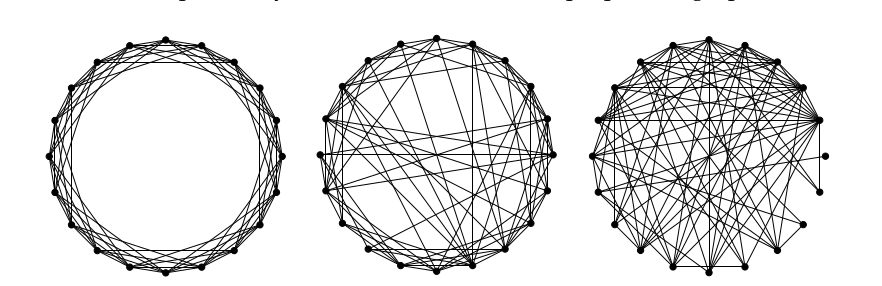
\includegraphics[width=0.9\linewidth]{figures/methodology/ws_graph}
	\caption{Watts and Strogatz graph model creation}
	\label{fig:erdist}
\end{figure}

Even though the small-world network model lacks the power-law degree distribution found in the real-world networks, it is an important model that motivated the research on random graphs. 

\subsection{Barab\' {a}si-Albert model}

The ER random graph model and WS small-world model are static models, where the number of nodes are fixed. It is one of the main reasons why they can not fully explain the properties of real systems. The size of real systems does not remain constant; real networks grow. Growth means that at each time step, new nodes are added to the network. The simplest model that produces the scale-free networks is Barabasi-Albert model.

\begin{itemize}
	\item The model starts from the small number of randomly connected nodes.
	\item Then at each time step, new node with $m_0$ links joins to the network. New node creates links with the nodes already present in the network, following the linking rules; i this model rules of preferential attachment. 
\end{itemize}
 
The preferential attachment is second important ingredient for generating system with scale-free properties. In the real-system the linking between nodes is not random process, there exists the preference toward specific types of nodes. For example the popular web-pages can easily get more visits or it is common that already popular papers will get more citations. This effect is also called rich-get-richer.

The simplest formulation of the preferential attachment model is that new nodes tend to connect with high degree nodes. The linking probability is then proportional to degree $k$:  

\begin{equation}
P(k_i) = \frac{k_i}{\sum_jk_j} 
\end{equation} 







\subsection{Nonlinear BA model}

\subsection{Aging model}

\subsection{Barabasi-Albert model}

The random network model differs from real networks in the two characteristics, growth and preferential attachment. In static models, number of nodes is fixed, while in growing models we try to simulate the continuous change in the system. More important ingredient, are linking rules. In real networks, new nodes tend to link to more connected nodes.

This model is defined as follows, we start from $m_0$ nodes, randomly connected, and at each timestep we add new node with m links that will connect to $m$ nodes already present in the network.  The probability that new node connects to node $i$ depends on node degree $k_i$ as

\begin{equation}
P(k_i) = \frac{k_i}{\sum_jk_j} 
\end{equation} 

New node can connect to any node in the network, however nodes with larger degree have higher probability to link new nodes. After time $t$ the model generates network with $N=t+m_0$ nodes and $m_0+mt$ links. Degree distribution is power-law with exponent $\gamma=3$. As network grows nodes with larger degree becomes bigger, so we end up with few nodes with many links, called hubs. Two simple mechanisms are responsible for emergence of scale-free networks. 

\textit{degree distribution}

To understand the emergence of scale-free properties we need to analyze the evolution of degree distribution. The rate at which an existing node get new links as result of new nodes connecting to it is

\begin{equation}
\frac{dk_i}{dt} = mP(k_i) = m\frac{k_i}{\sum_jk_j}
\end{equation}

each new node arrives with m links. The sum is $2mt - m$ so the equation for large t becomes:

\begin{equation}
\frac{dk_i}{k_i} = \frac{1}{2}\frac{dt}{t}
\end{equation}

solving this equation we get that degree of node in time step t is $k_i(t)=m(\frac{t}{t_i})^\beta$, where $\beta=1/2$. 

We note that degree of each node increase following power-law; the growth in degrees is sub linear, as each new node has more nodes to link than previous. The eirlier node $i$, the higher is its degree. Hubs are large as they arrived early in the network. 

In summary, the analytical calculations predict that the Barabási-Al-
bert model generates a scale-free network with degree exponent 3. The degree exponent is independent of the m and m 0 parameters. The degree distribution is stationary explaining how different systems have similar structural properties. 

In summary, the absence of preferential attachment leads to a growing network with a stationary but exponential degree distribution. In contrast the absence of growth leads to the loss of stationarity, forcing the network to converge to a complete graph. This failure of Models A and B to reproduce the empirically observed scale-free distribution indicates that growth and
preferential attachment are simultaneously needed for the emergence of the scale-free property.

In the past decade we witnessed the emergence of two philosophically different answers. The first one views preferential attachment as the interplay between random events and some structural property in the network. The second assumes that each new node or link balances conflicting needs. 

The BA model postulates the presence of preferential attachment. Yet, we can build models that generate scale free networks without preferential attachment. The link selection model offers the simplest mechanism that generates a scale-free network. At each time step we add new nodes to the network, we select link at random and connect the new node to one of the two nodes at the end. The higher is degree of the node, the higher is chance that node is located at the end of chosen link. The more k-degree nodes are there, the more likely is that k node is at the end of chosen link. Probability that node at the end of randomly choosen link has degree k is $q_k = Ckp_k$. The fact that bias is linear with k indicates that the link selection model builds scale-free networks. 
Copying model can also generate scale-free networks. In each time step a new node is added to the network. To decide where it connects we randomly select node u. Then with probability $p$ new node links to $u$, otherwise with probability $1-p$ we randomly choose an outgoing link of node $u$ and link the new node to its target. The likelihood that new node connects to degree-k node is $P(k)=\frac{p}{N} + \frac{1-p}{2L}k$, the second part is equivalent in selecting a node to randomly selected link. The popularity of the copying model lies in its relevance in real systems. It is common in social networks, citation networks or even protein interactions. 
in optimization, when new nodes balance conflicting criteria as they decide where to connect

\textit{diameter}
The network diameter, represents the maximum distance in the BA model, $d \sim \frac{lnN}{lnlnN}$. The diameter grows slower than $lnN$, making the distances in BA model smaller than in random graph. The difference is found for large N. 
\textit{clustering}
The clustering coefficient of the BA model follows $C \sim \frac{ln N^2}{N}$. It is different from clustering found in random networks, and BA networks are in general more clustered. 

\subsection{Nonlinear BA model}

In summary, nonlinear preferential attachment changes the degree
distribution, either limiting the size of the hubs $(\alpha < 1)$, or leading to su-
per-hubs ($\alpha > 1$, ). Consequently, $P(k)$ needs to depend strictly lin-
early on the degrees for the resulting network to have a pure power law p k .
While in many systems we do observe such a linear dependence, in others,
like the scientific collaboration network and the actor network, preferen-
tial attachment is sublinear. This nonlinear $P(k)$ is one reason the degree
distribution of real networks deviates from a pure power-law. Hence for
systems with sublinear  the stretched exponential (5.23) should offer a
better fit to the degree distribution.


In real systems preferential attachment can be more influenced by the age of the node. If parameter alpha is negative, ageing effect overcomes the role of preferential attachment, and scale-free properties are lost. For large negative alpha, the network turns into the chain, where the youngest nodes are the most attractive. On the other hand for a positive alpha, new nodes will link to older nodes. Positive alpha makes the network more heterogeneous, and scale-free nature still exist but exponent gamma is different from 3.  for the high alpha all nodes will tend to connect to oldest node. 

\subsection{Ageing model}

In the general ageing model, we have linking rules where rules connecting probability depends on both of node degree and age difference between new and old node.  With parameters alpha and beta we can control the structure of generated networks. I already talked about some limits of the general model. We saw that for specific parameters there are SF networks, BA model, if we move from that point SF behaviour with power-law with exponent 3 is lost. And other classes of networks can appear. In general, model, when alpha and beta are both positive, rich get richer phenomena is more promoted. On the other hand, the region where beta is positive and alpha negative can be interesting, because SF networks can appear only along the critical line. 

In growing network models is considered that at each time step one node is added to the network. The remaining question is if there is any change if network growth is not linear anymore and how does it influence the structure of obtained networks.  In this work, we use numerical simulations to explore the case when $M(t)$ is a correlated time-varying function and study how these properties influence the structure of generated networks for different values of parameter $-\infty<\alpha\leq-1$ and $\beta\geq1$ and constant $L$.












